\large{
Durante lo svolgimento di caso di studio, verrà ricreata, visualizzata e semplificata la struttura del grafo clusterizzato della \figurename{\ref{fig:springExample}}, utilizzato in precedenza a titolo di esempio per delucidare il lettore sulle forze in gioco tra cluster e nodi nel metodo spring-embedding. Inoltre sarà supposto che il cluster contenente tutto il resto del grafo sia definito come radice dell'albero di inclusione $T$.

\section{Creazione e modifica}
\begin{figure}[!htb]
	\begin{center}
		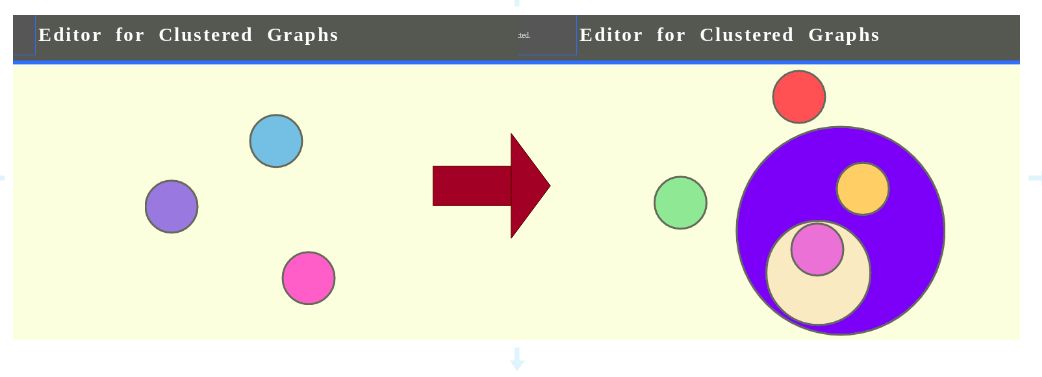
\includegraphics[width=1 \linewidth]{figure/prePostEdit}
	\end{center}
	\caption{I cluster pre e post inserimento dei sotto-cluster \label{fig:prePostEdit}}
\end{figure}
Dopo il log-in iniziale viene automaticamente creato il cluster radice, essendo rappresentato dal piano di lavoro \#cgraph stesso. Essendo un caso di studio del quale non si possiede un file json prestabilito ed essendo differente da ogni modello preimpostato del software, risulta necessaria la creazione partendo da una pagina bianca. Detto ciò anche l'oggetto \textit{clusteredGraph} sarà completamente vuoto e l'utente inizierà ad utilizzare il sistema partendo dalla creazione dei cluster di livello uno. Definiti questi oggetti si passerà alle interazioni per la creazioni dei cluster figli. In questo caso sarà necessaria dunque una interazione per ogni cluster figlio che si vorrà definire poiché ogni volta il sistema dovrà aggiornare la visualizzazione dei dati creati in quanto cambieranno il raggio $r_c \forall \mu$ cluster trasformato e nuove forze dovranno essere inserite. La creazione dei figli di un cluster può essere vista nella \figurename{\ref{fig:prePostEdit}} in cui si mette a confronto la visualizzazione dei dati antecedente e conseguente l'inserimento dei sotto-cluster. 
Come si nota, prima e dopo le operazioni di inserimento, sono state cambiate automaticamente dalla funzione di redraw le posizioni degli oggetti e manualmente, mediante una interazione da parte dell'utente, i colori degli oggetti mediante le interazioni già analizzate.Si passa ora all'introduzione di nodi e delle loro connessioni.
Avendo terminato le interazioni relative alla creazione degli elementi richiesti dal caso di studio si può passare ad eseguire operazioni di encode dei dati.
\newpage
\begin{figure}[!htb]
	\begin{center}
		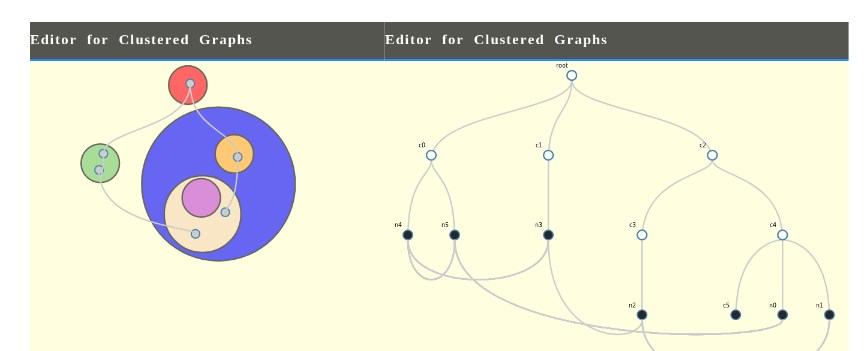
\includegraphics[width=1 \linewidth]{figure/views}
	\end{center}
	\caption{visualizzazione del grafo rappresentato nelle due visualizzazioni \label{fig:views}}
\end{figure}
Nella \figurename{\ref{fig:views}} è mostrato il compimento del grafo richiesto e della sua visualizzazione in entrambi gli encode disponibili. Si nota inoltre che vi è un cluster senza nodi e non connesso a nulla. L'utente può decidere di eliminarlo oppure lasciarlo nel caso di future modifiche magari inserendo un testo descrittivo per quel particolare elemento. Entrambe le operazioni sopra citate possono essere eseguite come mostrato nella figura \figurename{\ref{fig:deleteOrAddText}} in cui sono state eseguite l'operazione di rimozione dell'oggetto superfluo a sinistra oppure l'operazione di descrizione a destra. Nel caso in cui l'elemento in questione venga rimosso, il sistema eseguirà un ricalcolo del raggio $r_c$ e delle forze del modello Force-directed scelto per ritrovare una posizione di equilibrio, esattamente come descritto nel capitolo relativo alle primitive di interazione.Creato il grafo clusterizzato richiesto l'utente può salvare il suo lavoro in un file json che ne descrive la struttura. Salvando la sessione di lavoro nelle volte future in cui si dovranno eseguire modifiche o ulteriori creazioni di oggetti non sarà necessario ricreare completamente la struttura ma basterà caricare i progressi salvati nella sessione precedente risparmiando tempo ed imperfezioni.
\begin{figure}[!htb]
	\begin{center}
		\vspace{1cm}
		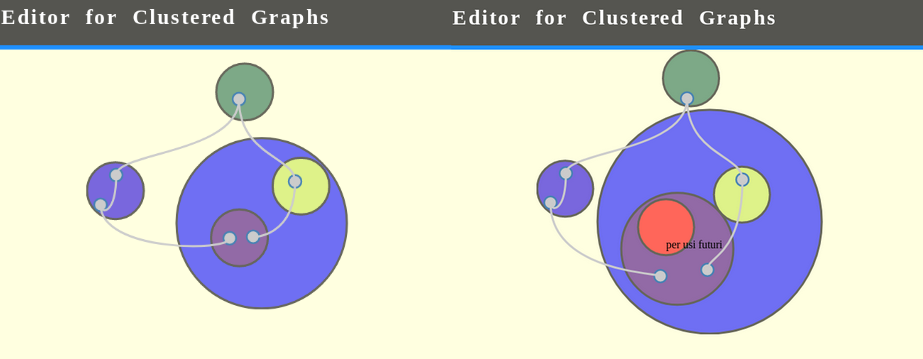
\includegraphics[width=1 \linewidth]{figure/deleteOrAddText}
	\end{center}
	\caption{Rimozione o aggiunta di un testo su un cluster\label{fig:deleteOrAddText}}
\end{figure}
\newline
Il file creato al salvataggio sarà lo stesso che in \figurename{\ref{fig:saveJson}} È inoltre possibile come già visto un salvataggio del grafo clusterizzato in un file con estensione .png. La resa della visualizzazione resta comunque il compito principale dell'utente ed è variabile al tempo impiegato per la creazione degli oggetti e per il loro posizionamento esatto. Per questo se si hanno esigenze specifiche riguardanti punti esatti e colorazioni predefinite si consiglia sempre di cominciare una sessione di lavoro su un piano vuoto.
\begin{figure}[!htb]
	\begin{center}
		\vspace{1cm}
		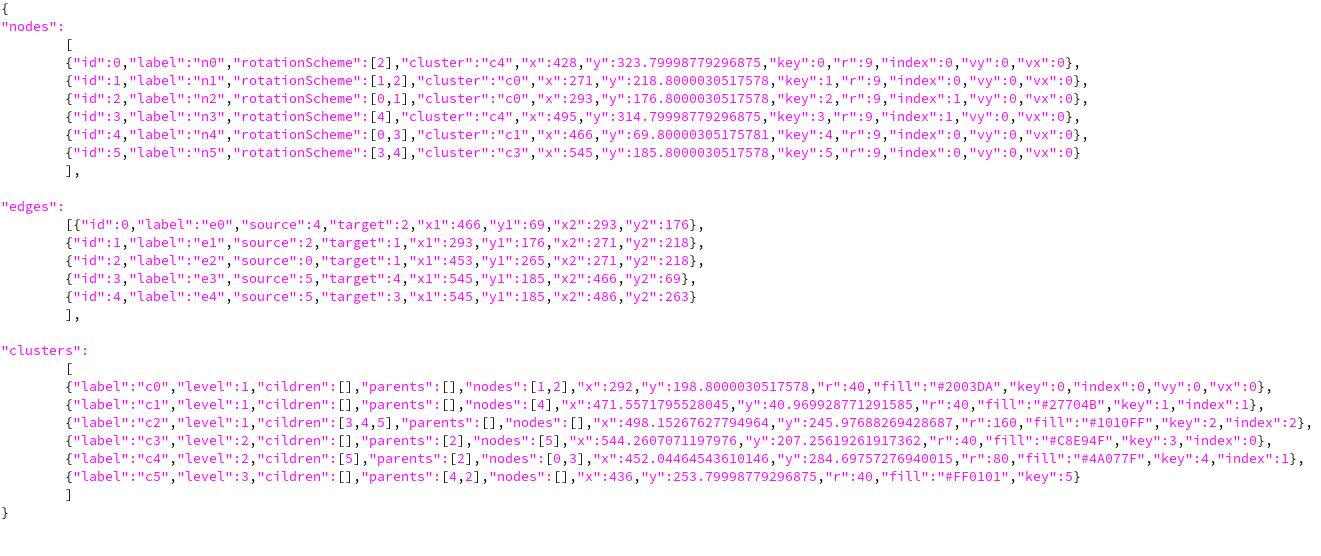
\includegraphics[width=1 \linewidth]{figure/saveJson}
	\end{center}
	\caption{Json riferito al salvataggio della struttura del caso di studio\label{fig:saveJson}}
\end{figure}
\newpage
\section{Riduzione e ripresa del grafo}
Terminate le operazioni inerenti la creazione e la modifica di un elemento o dell'intero grafo clusterizzato, l'utente decide di rendere il grafo della \figurename{\ref{fig:views}} flat. Supponendo poi che sia stato eliminato il cluster senza nodi in quanto non necessario alla visualizzazione, mediante una ulteriore interazione è possibile eseguire l'operazione vista nel capitolo precedente. Il risultato è quello mostrato nella figura \figurename{\ref{fig:treeAfterFlat}} mediante la quale si vede il risultato della semplificazione dell'istanza di grafo clusterizzato $C=<G,T>$ in una istanza $C_f=<G_f,T_f>$ con $T_f$ flat.
\begin{figure}[!htb]
	\begin{center}
		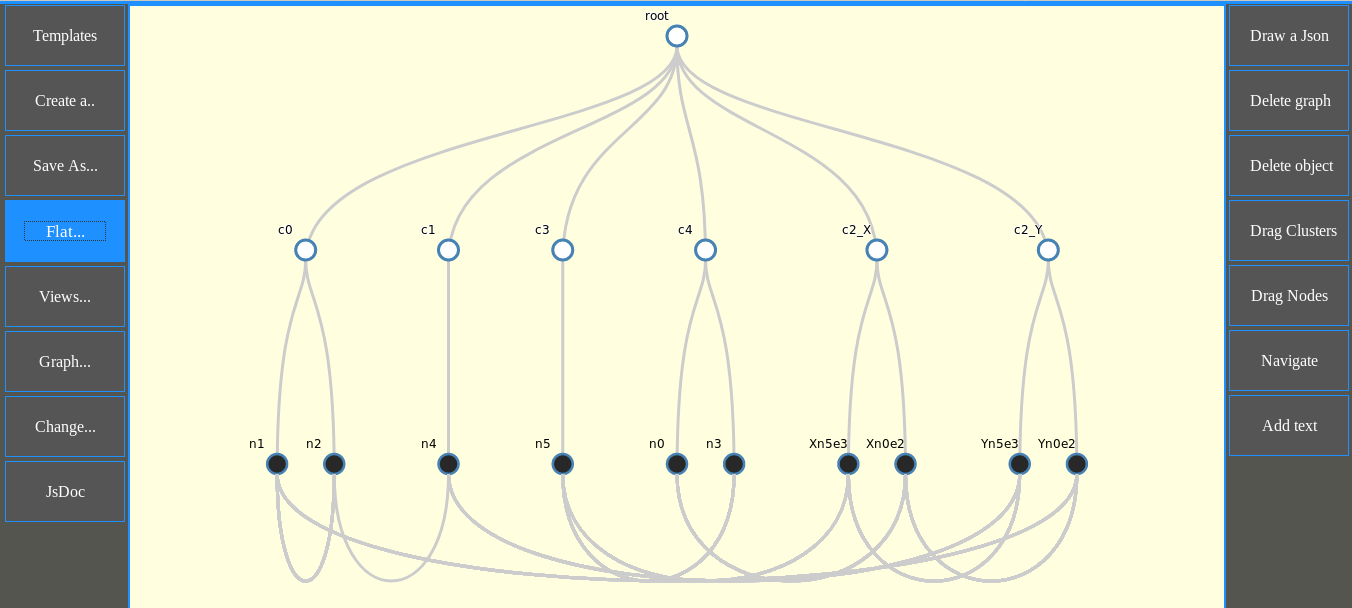
\includegraphics[width=0.8 \linewidth]{figure/treeAfterFlat}
	\end{center}
	\caption{Visione nella treeView dell'istanza flat del grafo clusterizzato\label{fig:treeAfterFlat}}
\end{figure}
A questo punto si ha la possibilità di procedere in due modi:
\begin{itemize}
	\item Analizzare l'istanza e salvare la struttura dati ricevuta sempre mediante file json come risultato ottenuto dalla sessione di lavoro;
	\item Ritornare allo stato della sessione precedente quella ottenuta dall'operazione di semplificazione.
\end{itemize}

È infatti possibile per l'utente continuare la modifica del grafo e ritornare ad avere i dati e la conseguente visualizzazione precedenti l'operazione di riduzione nell'istanza equivalente. Questo è possibile poiché, come visto nel capitolo precedente, durante il primo passo dell'algoritmo di semplificazione, si esegue il salvataggio dei dati relativi all'ultima visualizzazione antecedente la riduzione in grafo clusterizzato flat rendendo l'interazione relativa all'operazione di semplificazione binaria On/Off. Analizzando la graphView dopo la flattizzazione il risultato sarà non dissimile da quello riportato nella \figurename{\ref{fig:graphAfterFlat}}.

\begin{figure}[!htb]
	\begin{center}
		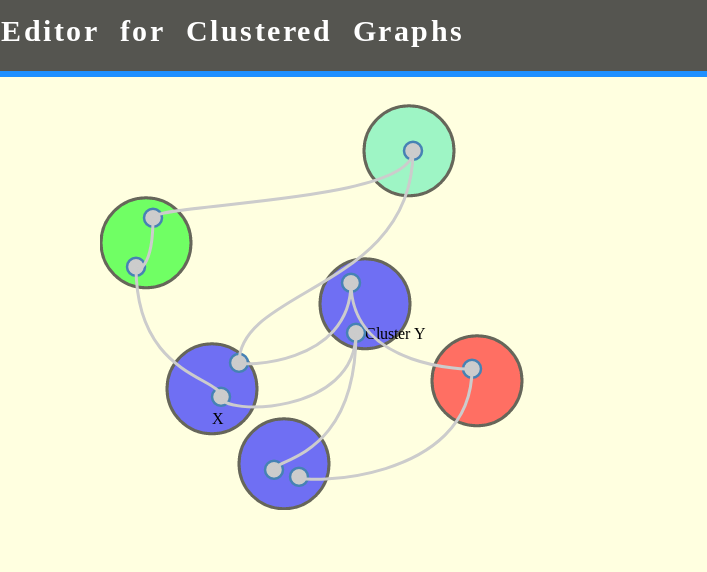
\includegraphics[width=0.9 \linewidth]{figure/graphAfterFlat}
	\end{center}
	\caption{Visione nella graphView dell'istanza flat del grafo clusterizzato\label{fig:graphAfterFlat}}
\end{figure} 
}